\documentclass[UTF8]{ctexart}
\usepackage{amsfonts}
\usepackage{amsmath}
\usepackage{amssymb}
\usepackage{amsthm}
\usepackage{booktabs}
\usepackage{color}
\usepackage{courier}
\usepackage{float}
\usepackage{geometry}
\usepackage{graphicx}
\usepackage{graphics}
\usepackage{hyperref}
\usepackage{listings}

\geometry{left=2.54cm,right=2.54cm,top=2.18cm,bottom=3.18cm}
\graphicspath{{./img/}}

\newcommand{\red}{\textcolor[rgb]{1.00,0.00,0.00}}

\begin{document}

\title{\textbf{HRPT数字卫星云图信号接收}}
\author{无44 \ 姜宏伟 \ 2014011041\\
        无46 \ 杨志坚 \ 2014011183\\
        无46 \ 严靖凯 \ 2014011192\\
        无46 \ 黄秀峰 \ 2014011193\\
        无48 \ 黄佳新 \ 2014011248}
\date{}
\maketitle

\section{背景}

卫星云图接收是电子系统设计中的一个经典项目。在传统的卫星云图信号接收中,人们通常选择接收美国国家海洋和大气局(NOAA)于20世纪中期发射的气象卫星NOAA-15,16,17,因为其发送的信号未进行复杂的编码,且频段较易接收。截止至今日,这三颗卫星中只有NOAA-17还在工作,因此本实验中考虑对该卫星发送的信号进行接收。

NOAA-17卫星所发送的信号包含多路信号,其中最常用且重要的为APT(Automatic Picture Transmission)信号和HRPT(High-Resolution Picture Transmission)。两路信号所传输的内容一致,但图像的分辨率不同,信号的频段、带宽、编码方式等也不同。APT信号的下行频率约为137.7MHz。该频率的信号可以通过软件无线电(SDR)直接接收与解码,并利用WXtoImg等软件直接显示。这是目前大多数卫星云图信号接收系统所采用的信号。HRPT信号的下行频率约为1.70GHz,由于频段过高,无法直接采用SDR接收。APT信号的接收已被广泛研究,不具有任何挑战性,因此我们在本实验中主要考虑对HRPT数字卫星云图信号的接收。

\section{系统框架}

我们设计的系统框架如下图:
\begin{figure}[H]
        \centering
        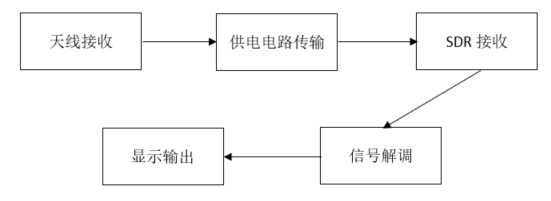
\includegraphics[width=0.7\textwidth]{images//framework.png}
\end{figure}

其中,天线接收部分利用主楼楼顶的卫星天线,供电电路需要自行设计制作,SDR接收利用现有的仪器实现,信号解调通过设计合适的方式实现,显示输出部分实现类似WXtoImg的功能。以下几节详细介绍了各模块的实现。

\section{HRPT信号解调}

为了对HRPS信号进行接收处理,我们首先查阅了NOAA-17卫星的数据手册与用户说明,了解了其数据制式与编码方式。HRPT信号将8bit的数字图像数据进行相位调制,其中符号0用前半周期为$+68^\circ$,后半周期为$-68^\circ$的调相信号表示;符号1用前半周期为$-68^\circ$,后半周期为$+68^\circ$的调相信号表示。传输的比特率为665400bit/s。

假设我们已完成了HRPT信号的接收,此时需要进行相位解调。相位解调的传统方法需要利用本地的同步载波,但由于卫星信号在传输过程中的多普勒频移等因素,同步解调将非常困难,因此需要采用其他方法。我们采用以下无需同步载波的方法:

假设待解调的调相信号为
$$
f(t) = A\cos(\omega t+\varphi(t)),
$$
其中$\varphi(t)$为时变的调相部分。我们考虑采用任意相位(无需同步)的正弦与余弦本地载波
\begin{align}
  \nonumber
  g_1(t) &= A\cos(\omega t+\psi),\\
  \nonumber
  g_2(t) &= A\sin(\omega t+\psi).
\end{align}
将$g_1(t)$余$g_2(t)$分别与$f(t)$相乘,得到
\begin{align}
  \nonumber
  f(t)g_1(t) &= A^2 \cos(\omega t+\varphi(t)) \cos(\omega t+\psi) \\
  \nonumber
  &= \frac{A^2}{2} \left( \cos(2\omega t+\varphi(t)+\psi) + \cos(\varphi(t)-\psi) \right), \\
  \nonumber
  f(t)g_2(t) &= A^2 \cos(\omega t+\varphi(t)) \sin(\omega t+\psi) \\
  \nonumber
  &= \frac{A^2}{2} \left( \sin(2\omega t+\varphi(t)+\psi) - \sin(\varphi(t)-\psi) \right).
\end{align}
注意分解出的两项,分别为频率为$2\omega$的高频分量与常数分量。在一个符号周期内进行积分,由于比特率665400bit/s远低于载波频率1.70GHz,故高频分量的积分结果将约等于0。因此我们有
$$
\frac{\int_{t_0}^{t_0+T}f(t)g_1(t)}{\int_{t_0}^{t_0+T}f(t)g_2(t)} \approx - \tan(\varphi(t)-\psi).
$$
此时,再利用$\arctan$并进行相位的unwrap,便可以得到$\varphi(t)-\psi$的值。

值得说明的是,此时便足以对信号进行解调,$\psi$的取值并无影响。这是因为这里的相位调制采用的是$68^\circ$而非$90^\circ$,可以通过两个值的相对位置关系进行判断。倘若相位调制采用的是$90^\circ$,则无法通过此方式解调,必须使用同步载波。

\section{放大电路设计}

\section{使用信号发生器模拟发送}

在完成了放大电路模块后,我们利用接收天线尝试了对HRPT信号的接收,但发现由于天线状态不佳、信号自身信噪比较差等因素,所接收的信号几乎无法复原。由于该困难相对难以克服,需要更好的接收天线等条件,因此我们不得已而选择对NOAA-17所发送的信号进行模拟发送,并进行接收与解调。为此,我们研究了HRPT信号发送的编码方式,然后逆向生成了发送数据,并用信号发生器和SDR模拟发送。

本次实验使用SFU信号源作为信号发生器,使用WinIQSIM和IQWizard处理数据生成.wv文件用于信号源生成信号,具体流程如下。

\subsection{用Matlab处理数据生成mat文件}

首先用Matlab处理我们要发送的数据,生成需要发送的I、Q两路信号数组(数值在-1至1之间),将数据保存为single类型(注意,如果不保存single类型,IQWizard在读取时会出错)。最后通过$$save('data.mat','-v6',I,Q)$$将数据存储为mat文件

\subsection{用WinIQSIM和IQWizard生成wv文件}

利用WinIQSIM和IQWizard可以将mat文件转化为信号源可读取的mv文件。

首先利用端口通信连接WinIQSIM和IQWizard

\begin{figure}[H]
        \centering
        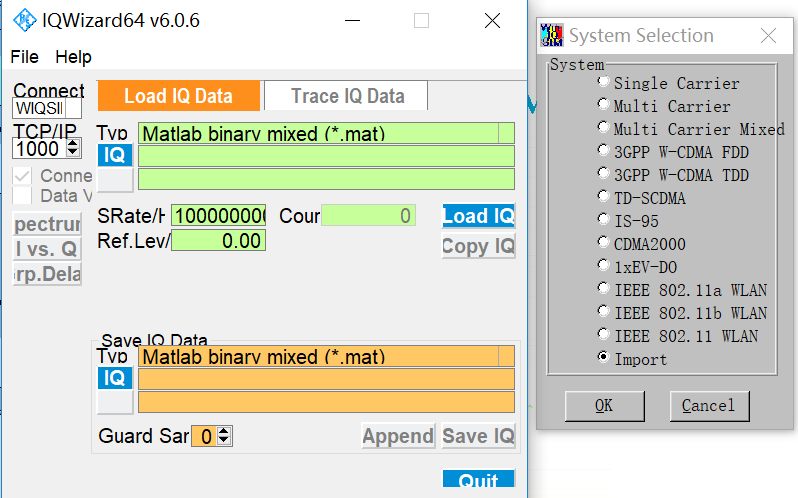
\includegraphics[width=0.9\textwidth]{images//connect.png}
\end{figure}

将mat文件导入到IQWizard中

\begin{figure}[H]
        \centering
        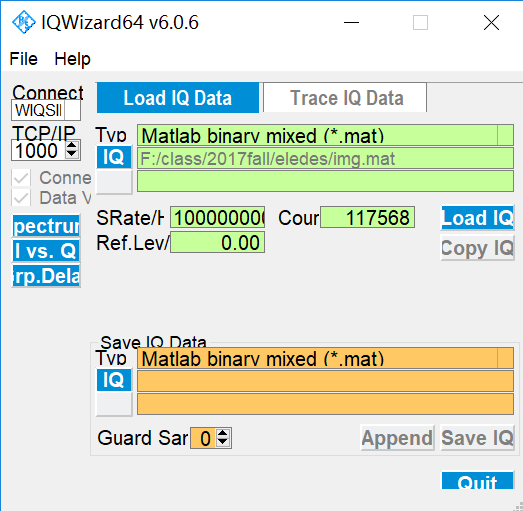
\includegraphics[width=0.7\textwidth]{images//loadmat.png}
\end{figure}

将数据从IQWizard传输到WinIQSIM

\begin{figure}[H]
        \centering
        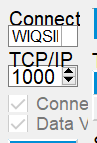
\includegraphics[width=0.2\textwidth]{images//transform.png}
\end{figure}

利用WinIQSIM将数据导出为SFU可读取的wv文件

\begin{figure}[H]
        \centering
        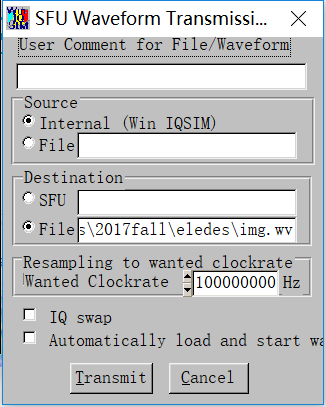
\includegraphics[width=0.4\textwidth]{images//getwv.png}
\end{figure}

\subsection{使用SFU信号源发送信号}

选择SIGNAL SOURCE为ARB

\begin{figure}[H]
        \centering
        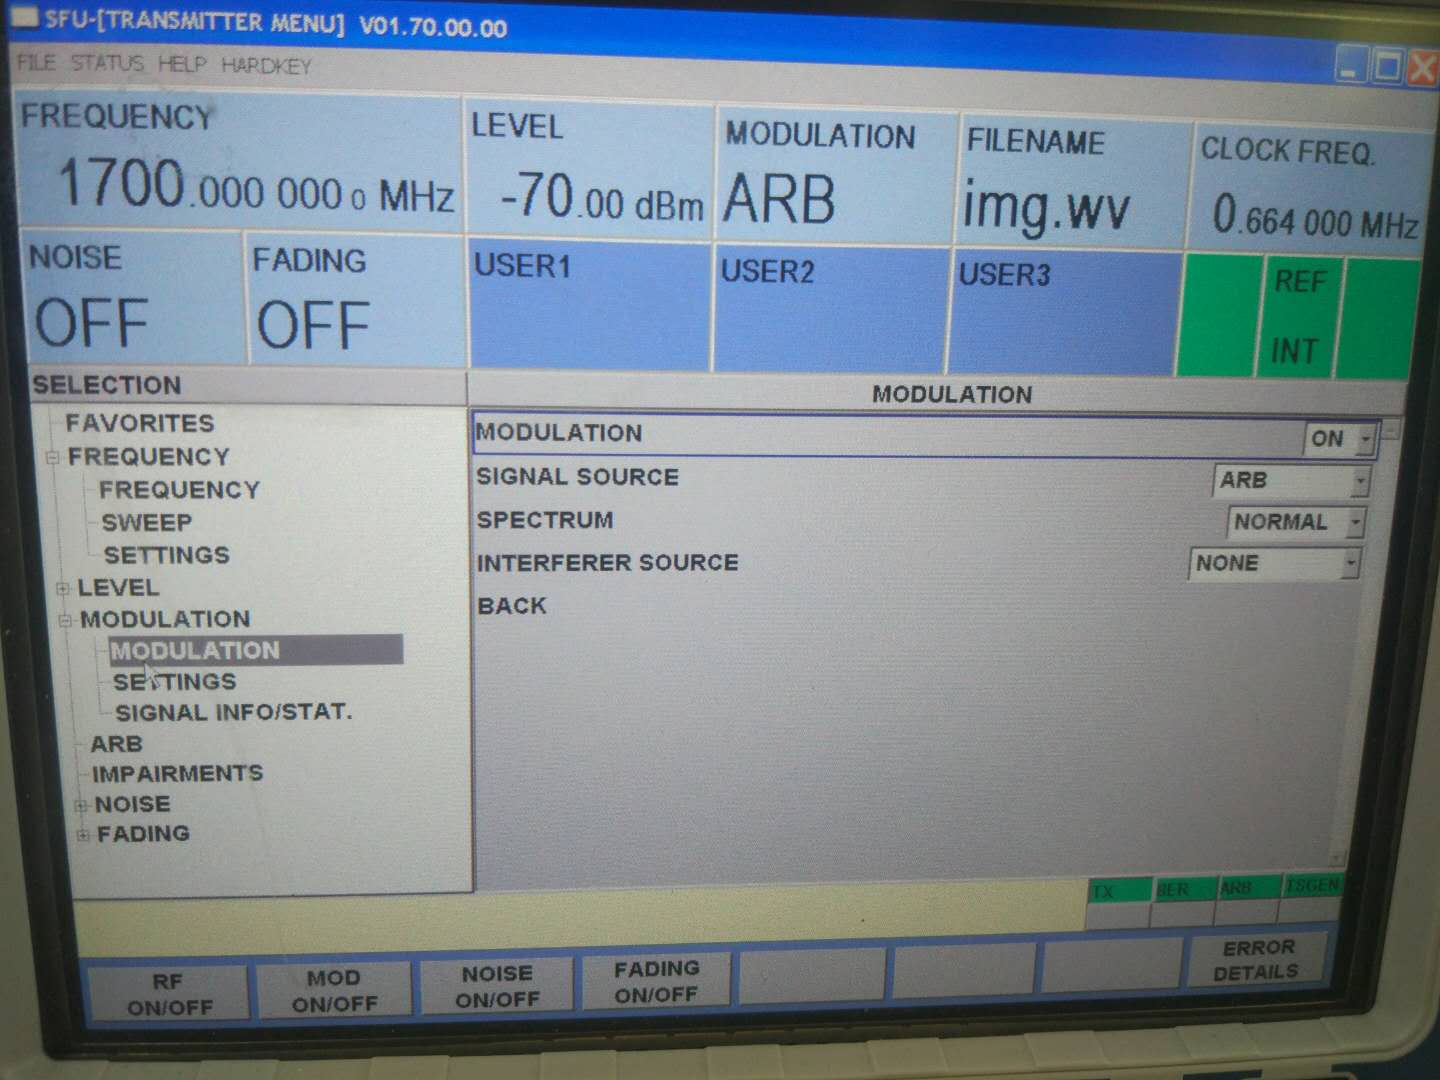
\includegraphics[width=0.8\textwidth]{images//setARB.jpg}
\end{figure}

导入wv文件

\begin{figure}[H]
        \centering
        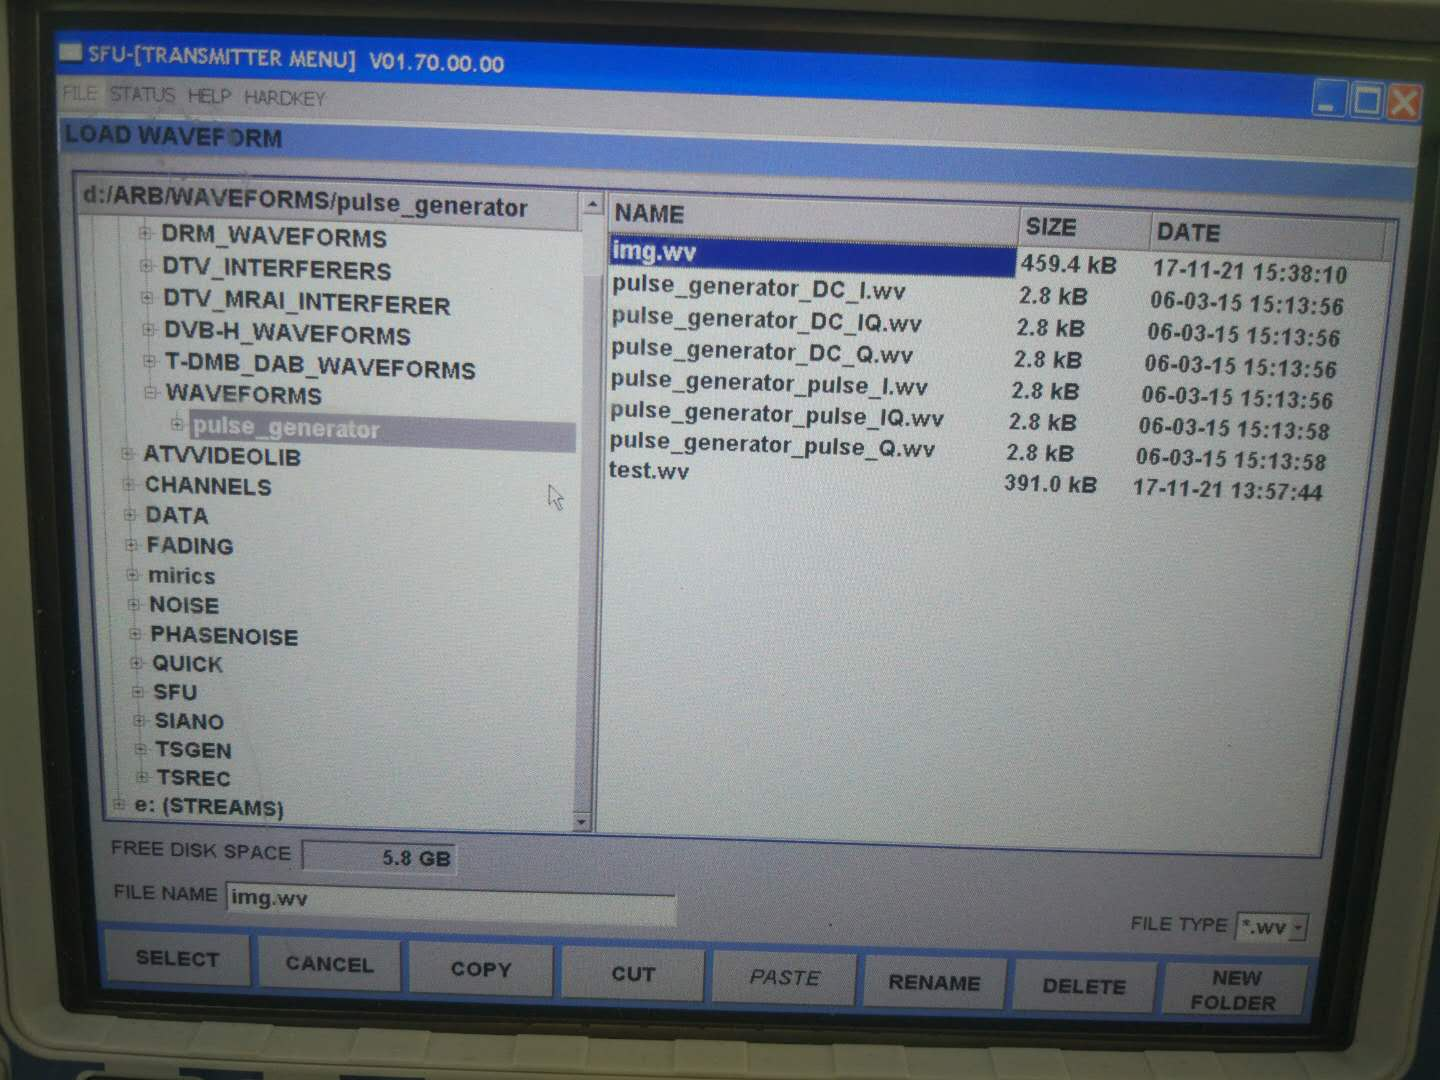
\includegraphics[width=0.8\textwidth]{images//loadwv.jpg}
\end{figure}

选择载波频率

\begin{figure}[H]
        \centering
        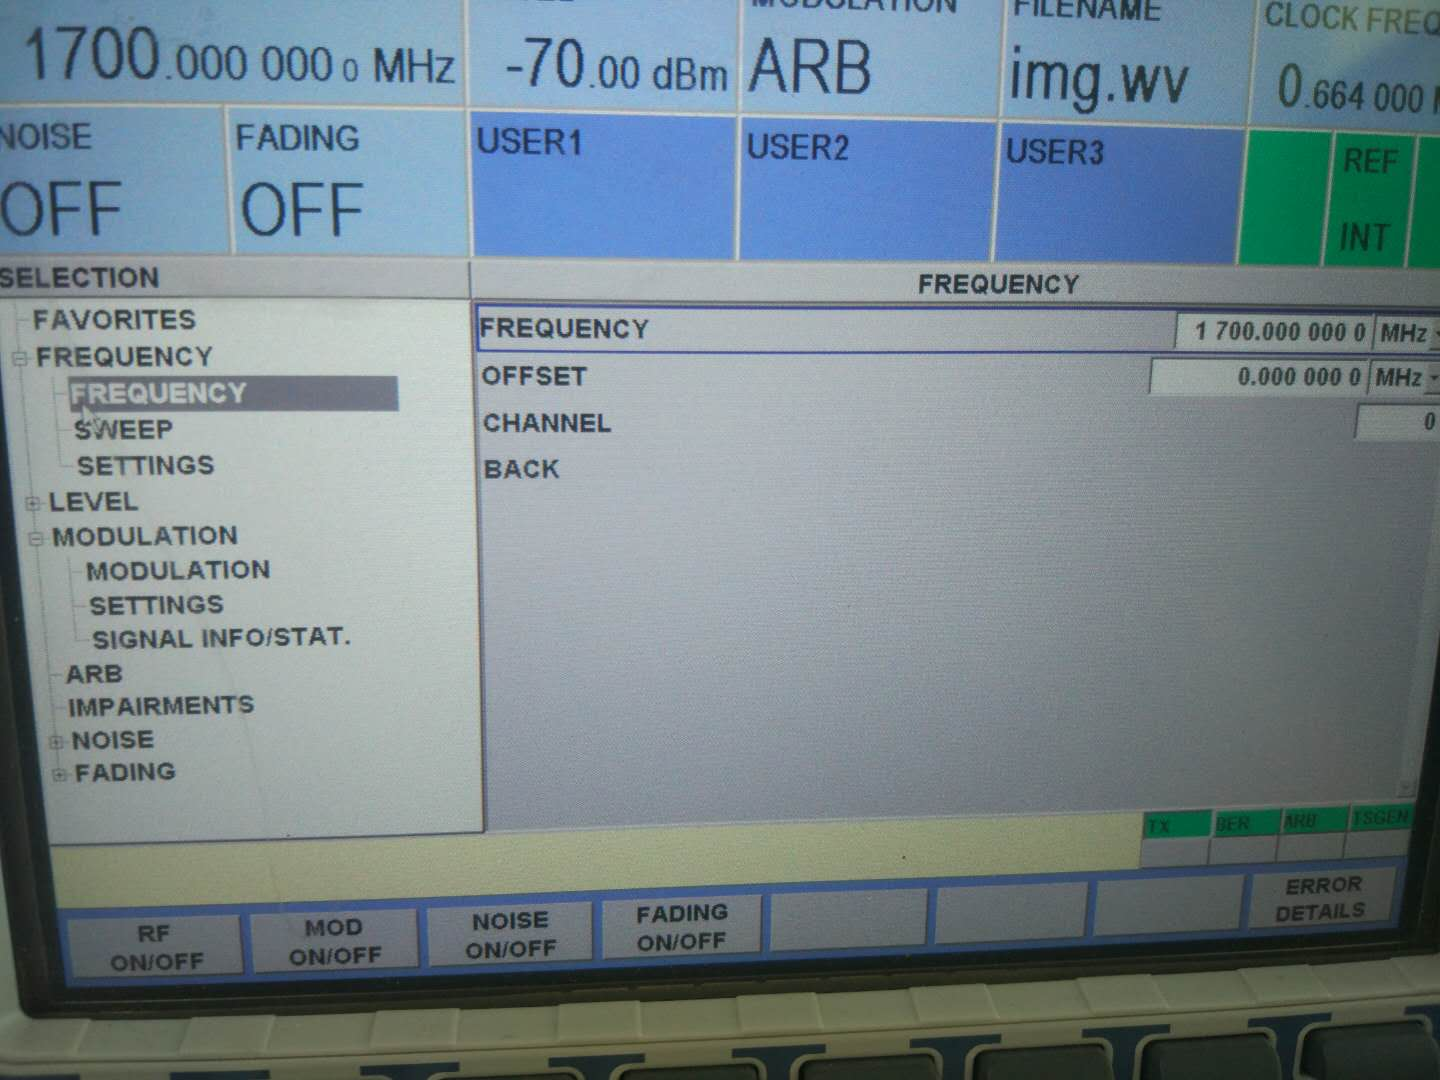
\includegraphics[width=0.8\textwidth]{images//setfreq.jpg}
\end{figure}

设置成功后,会循环发送wv文件中的信号。

\section{测试结果}

\section{分析与讨论}


\end{document} 